\documentclass{article}

\usepackage{geometry}
\geometry{margin=1in}


\usepackage{amsfonts}
\usepackage{amsmath}
\usepackage{bbm}

\usepackage{graphicx}
\usepackage{subcaption}

\usepackage{multirow}

\usepackage{hyperref}

\usepackage{natbib}
\bibliographystyle{plainnat}

\usepackage{xcolor}
\newcommand{\todo}[1]{{\color{orange}{TODO: #1}}}
\newcommand{\note}[1]{{\color{blue}{NOTE: #1}}}
\newcommand{\gur}[1]{{\color{teal}{Gur: #1}}}
\newcommand{\yarden}[1]{{\color{magenta}{Yarden: #1}}}


\title{The Effect of Age of Enrollment on the Probability of Graduating from Academic Programs}
\author{Gur Keinan 213635899 \and Yarden Adi 212585848}
\date{October 30, 2024}


\begin{document}

\maketitle

\begin{abstract}
    Many adolescents worldwide have wondered when they should start their journey in higher education. The writers of this project themselves had decided long ago to join the 'Atuda' program, which means starting university at the relatively young age of eighteen. Thus, it is natural to wonder - does the student's age at the start of learning at the university affect the success of the student? An answer to this question can drastically change the landscape of the campuses worldwide and the grades of those studying there. In this Causal Inference project, we aim to explore precisely that. Specifically, we investigate the following causal question: \emph{What is the causal effect of enrolling as an adult student (age 21 or older) on the probability of graduating from an academic program within the allotted time?} Throughout this project, we present and explore the data we use to tackle this question and determine its suitability for causal analysis tasks, formally present the methods we use to answer the research question, present and discuss the analysis results, and conclude the project. One can find all of the resources used in the project in this \href{https://github.com/GurKeinan/Causal-Inference-Project-Effect-of-Age-on-Graduating}{GitHub repository}.
\end{abstract}

% \textbf{Note on AI Usage:} We did not use generative AI to write this report. We only used ChatGPT, Claude, and Grammarly to revise and correct our writing.

\section{Data Review and Preprocessing}

\gur{Opening sentence.}

\subsection{Data Review}

The data used in our project originated from research done in Portugal by the \href{https://www.ipportalegre.pt/pt/}{Polytechnic Institute of Portalegre} (higher education institute that focuses on technology), as an attempt to provide information to the tutoring team about the risk of students' dropout and failure \citep{data7110146}. Commonly, it is used to build machine learning models for predicting academic performance and dropout (see relevant \href{https://www.kaggle.com/datasets/ankanhore545/dropout-or-academic-success/data}{Kaggle competitions in this subject}).

The data contains information about students' pre-academic background, age, academic performance, social and economic status, and other relevant variables. It consists of 4424 records and 37 variables, including the enrollment age. The dataset includes a trinary outcome variable indicating whether a student dropped out, graduated, or is still enrolled in the academic program. 

The data was created by joining three primary data sources: 
\begin{enumerate}
    \item CNAES (National Competition for Access to Higher Education) - contains information about students' academic backgrounds, demographics, and course applications at the time of their enrollment in Portuguese higher education institutions.
    \item AMS (Academic Management System) - provides student records data, including demographic information, course enrollments, and academic performance throughout their studies.
    \item PORDATA (Contemporary Portugal Database) - provides macroeconomic data, including unemployment, inflation, and GDP figures.
\end{enumerate}

Traditionally, each attribute used in the dataset belongs to one of the following classes: demographic,
socioeconomic, macroeconomic, academic data at enrollment, and academic data at the end of the first and second semesters. For a full list of the variables in the dataset and their corresponding classes, please refer to Table~\ref{table:variables list}

\subsection{Data Preprocessing}

\gur{removal of application mode 39 because it is too similar to treatment}

\paragraph{Treatment and Target variables} Following our causal question, we introduce a new binary variable - "being 21 or older". This variable acts as the \emph{treatment variable} in our analysis. We omit the numerical age variable for the rest of the analysis. Additionally, as our question focuses on the probability of graduating from an academic program within the allotted time, we introduce another binary variable - "Graduated from an academic program within the expected timeframe" rather than the commonly used trinary variable - "graduate/ enrolled/ dropout". This variable is the \emph{target variable} in our analysis. Importantly, we consider students who are still enrolled beyond the expected completion time as not having graduated within the allotted time, aligning with the standard duration of academic programs in Portuguese higher education. The distributions of the target and treatment variables are visually presented in Figure~\ref{fig:target_and_treatments_histograms}

\begin{figure}
    \centering
    \caption{Distributions of the target (graduation within allotted time) and treatment (adult enrollment) variables}
    \label{fig:target_and_treatments_histograms}
    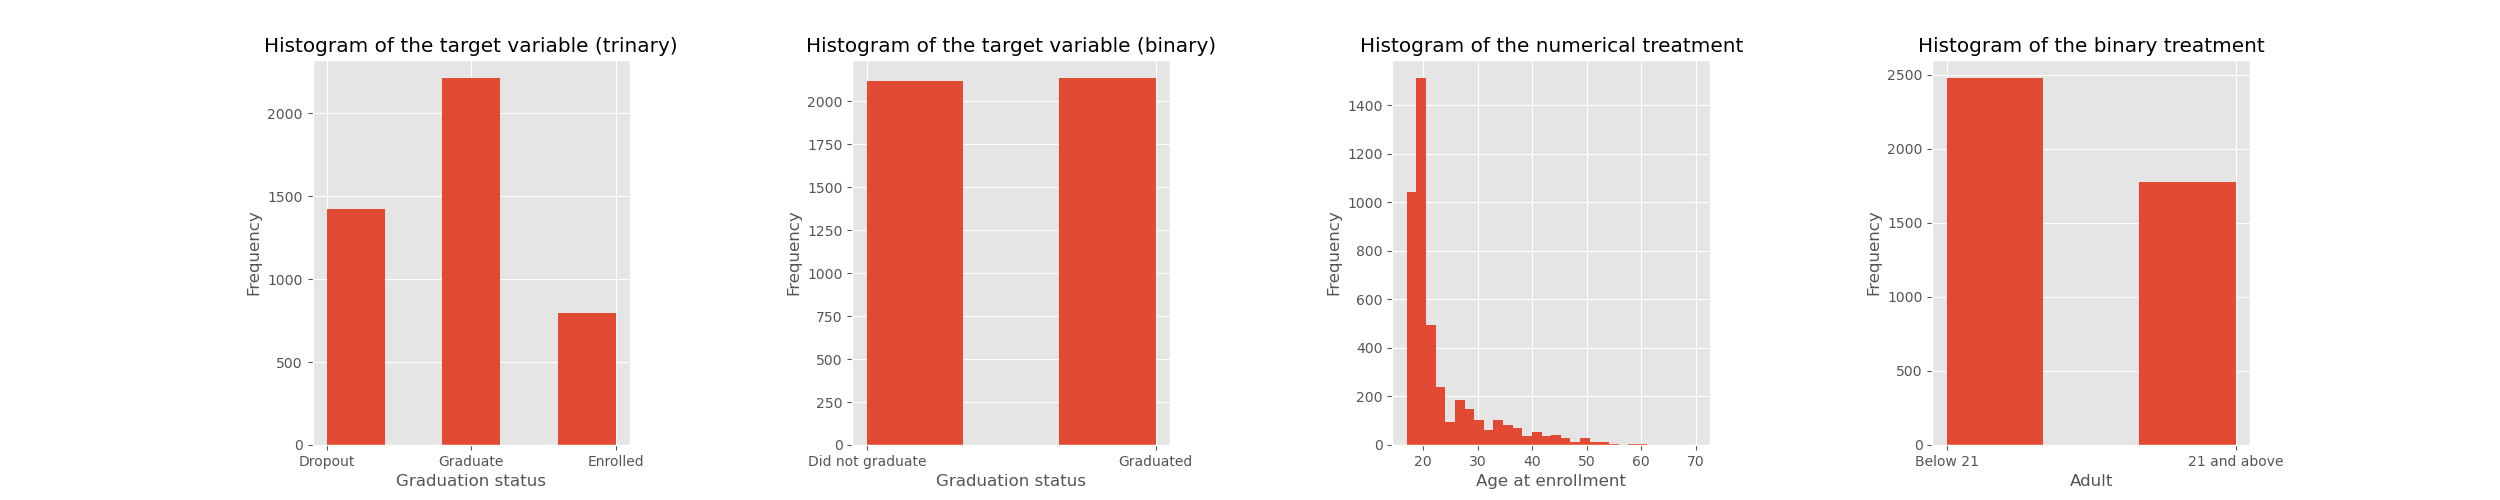
\includegraphics[width = \textwidth]{plots/target_and_treatments_histograms.png}
\end{figure}

\paragraph{Removal of post-treatment variables} The dataset contains multiple variables that had been gathered throughout the students' academic journey, e.g., academic accomplishments, debts, and payment tracking. \yarden{I would write \textbf{despite being informative} instead of \textbf{although informative}} Although informative for machine learning models trying to predict academic dropout, these accomplishments were recorded after the treatment was determined and, therefore, cannot be safely used in the causal inference procedure. We eliminated those variables to maintain the integrity of our results and prevent any post-treatment interference.

\paragraph{Clustering categorical values} The dataset is of impressive complexity and detail, as evident by the categorical variables with over 30 unique values. To perform meaningful analysis, we manually cluster similar categories into one broader category to represent them instead of simply removing the less frequent value. For example, we merged the values 'Armed Forces Professions', 'Armed Forces Officers', and 'Armed Forces Sergeants' into a single 'Armed Forces' value. We performed this procedure on five variables within the data set - the qualifications and occupations of the parents (mother and father) and the student's previous qualifications. 

\paragraph{Pruning categorical outliers} Even after performing the previous step, some variables still contained rare values. After careful consideration and visual inspections, we decided to prune some of the rare values to ease the analysis. The pruning resulted in a sample exclusively consisting of individuals with Portuguese nationality, which may limit the generalizability of this study to a broader population. 

\todo{scaling and encoding - I think that it can come later on in the analysis part, but don't forget!}

After the preprocessing stage, the dataset comprises 4249 records, with each record containing 21 variables. Among these variables, 5 are numerical and the rest are categorical.


\section{Assumptions for Causal Inference}\label{sec:assumptions}

In this section, we formally present and discuss four assumptions regarding the nature of our data. Combined, those assumptions guarantee the trustworthiness of an observational causal experiment's results.

\subsection{Stable Unit Treatment Value Assumption (SUTVA)}

The SUTVA assumption consists of two parts. The first one is \emph{no interference}, which requires that the potential outcomes of each unit are not affected by the treatment assignment of any other unit; the second is \emph{no hidden variations of treatment}, which forbids the existence of different forms or versions of each treatment level, which lead to different potential outcomes.

In our experiment, the treatment variable, 'enrolling as an adult student (over 21)' \gur{is it?}, is well-defined and has only two versions. Hence, the second part of the assumption safely holds. The assumption's first part holds if we presume one student's adulthood does not affect the probability of his fellow student graduating from the program, which is controversial. There are several aspects in which the varied spectrum of ages on the campus might affect the students' success. Such elements include but are not limited to 1) peer effects - encountering different perspectives and learning methods (that can be related to one's age) might affect one's abilities; and 2) In competitive programs, students' success may be directly affected by their peers' accomplishments. Therefore, if age is indeed related to one's academic achievements, one student's age can indeed affect another's success.

\subsection{Consistency}

The Consistency assumption states that an individual's potential outcome under his or her observed exposure history is the outcome that will actually be observed for that person. Put formally, for a unit that receives treatment $T$, we observe the corresponding potential outcome $Y = TY_1 + (1-T)Y_0$. This assumption can be violated when the individual's history is misreported. Since our data was extracted from credible and regulated sources and processed using careful and documented manipulations, we believe that the Consistency assumption likely holds in our study. 

\gur{elaborate more? Data Source Reliability, Clear Treatment Definition, Outcome Measurement, Data Processing Transparency, Stable Treatment}


\subsection{Ignorability - No Unmeasured Confounders}

% The Ignorability assumption states that the treatment assignment $T$ is independent of the potential outcomes $Y_0, Y_1$ given the observed covariates $X$, i.e., $Y_0, Y_1 \perp T \ | \ X$. 

% \gur{'Unverifiable assumption.' https://www.ncbi.nlm.nih.gov/pmc/articles/PMC10666970/}

% \gur{'We close with a reminder to readers of the optimistic view of the complexity of data and how the correlation between observed variables and unmeasured ones can reduce any bias associated with unmeasured information.' https://www.ncbi.nlm.nih.gov/pmc/articles/PMC10666970/}

% \gur{something about stress and events during the studies that weren't documented?}

The ignorability assumption, also known as the assumption of no unmeasured confounders, states that the treatment assignment \( T \) is independent of the potential outcomes \( Y_0, Y_1 \) given the observed covariates \( X \), that is, \( Y_0, Y_1 \perp T \ | \ X \). This assumption is essential for ensuring that the estimated treatment effect is unbiased and not confounded by factors affecting both the treatment and the outcome.

However, this assumption is inherently unverifiable in practice since it is impossible to confirm whether all relevant confounders have been measured and included in the model. As noted by \citet{hernan2006estimating}, we cannot account for unmeasured confounders, as we do not observe them. Despite this limitation, research has shown that correlations between observed covariates and unmeasured confounders can reduce the bias associated with missing information \citep{schulz2023no}. This means that if our dataset contains variables from diverse domains that possibly affect the treatment or potential outcomes, we may mitigate the effect of unmeasured confounders.

Based on \citet{alyahyan2020predicting}, we identify several potential confounder groups that may affect both age of enrollment and the probability of academic success: pre-academic performance (such as high school grades, admission test results, and previous course grades); student demographics (including gender, race/ethnicity, socioeconomic status, and family background); student environment (such as class type, semester length, and type of program); and psychological factors (such as student interest, study behavior, stress, anxiety, time management, self-regulation, and motivation). In addition to these factors, macroeconomic indicators, like unemployment rates and inflation, are also considered necessary.

Our dataset contains most of the relevant classes of confounders, including pre-academic performance, student demographics, student environment, and macroeconomic indicators. However, we lack psychological factors, which could be a significant limitation in our analysis, as these factors may influence both age of enrollment and academic success. Furthermore, although academic progression is also an essential confounder, it is a post-treatment variable and, therefore, cannot be used in the causal analysis without risking post-treatment bias.

\subsection{Common Support (Overlap)}

The Common Support assumption states that each unit has a non-zero probability of receiving each treatment level, i.e., $\forall x \in X, P(T=1|X=x) > 0$ and $P(T=0|X=x) > 0$.

We empirically validate this assumption using propensity scores. We trained a logistic regression model to predict the treatment assignment based on the covariates and used the predicted probabilities as the propensity scores. We then plotted the propensity scores of the treated and control groups to ensure a significant overlap between the two groups. The results are presented in Figure \ref{fig:common_support}. The lowest predicted propensity score of the treated group is $0.0209$, and the control group's is $0.009$. Therefore, we conclude that the common support assumption holds in our data.

However, it is essential to note that not everyone receives similar opportunities to acquire higher education in Portugal. According to the OECD Review of Inclusive Education in Portugal \citep{/content/publication/a9c95902-en}, despite significant improvements in access and attainment, inclusion challenges persist for disadvantaged groups such as low-income students and those with immigrant backgrounds. 

These disparities suggest that while there may be overall support for the common support assumption, certain groups might have systematically different opportunities or probabilities of accessing higher education and, therefore, receiving the treatment. This might pose a challenge to the common support assumption, particularly for vulnerable populations.


\begin{figure}
    \centering
    \caption{Common support of the propensity scores}
    \label{fig:common_support}
    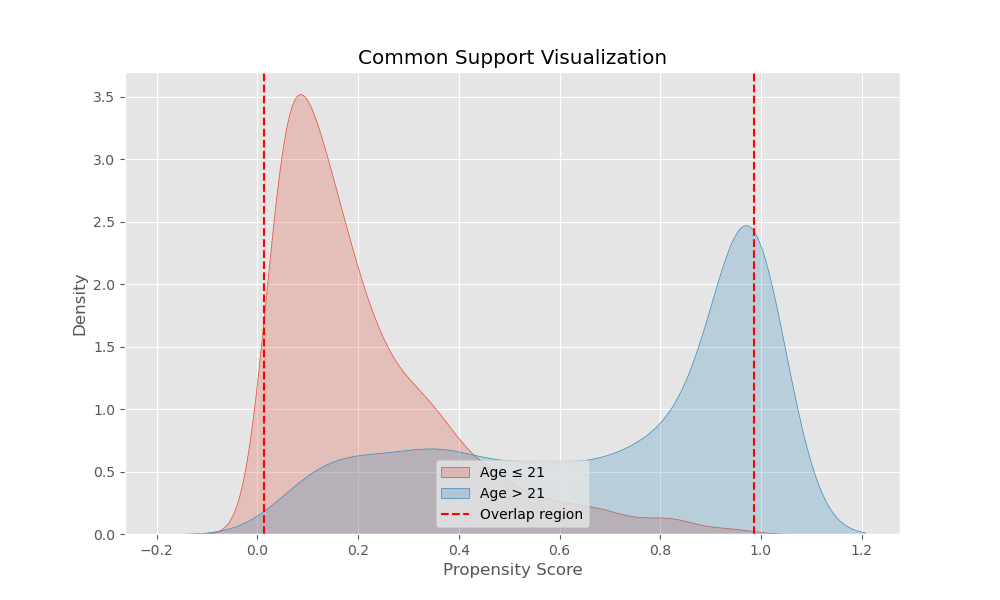
\includegraphics[width = 0.8\textwidth]{plots/common_support.png}
\end{figure}



\section{Causal Analysis Methodology}

After validating the assumptions for causal inference, we describe the methodology used to perform the causal analysis. We present the relevant measures of causal effects and the methods we use to estimate them.

\subsection{Measures}

To quantify the causal effect of the treatment on the outcome, one usually tries to estimate the Average Treatment Effect (ATE). However, in some cases, estimating the Average Treatment Effect on the Treated (ATT) or the Average Treatment Effect on the Control (ATC) is more informative. We formally present those measures below.

\paragraph{Average Treatment Effect (ATE)} Defined as the difference between the expected outcome under treatment and the expected outcome under control. Formally, it is defined as $ATE = E[Y_1 - Y_0]$.

\paragraph{Average Treatment Effect on the Treated (ATT)} Defined as the difference between the expected outcome under treatment and the expected outcome under control, but only for the treated units. Formally, it is defined as $ATT = E[Y_1 - Y_0 | T = 1]$. 

\paragraph{Average Treatment Effect on the Control (ATC)} Defined as the difference between the expected outcome under treatment and the expected outcome under control, but only for the control units. Formally, it is defined as $ATC = E[Y_1 - Y_0 | T = 0]$. 

Each of the three measures provides a different perspective on the causal effect of the treatment. The ATE measures the average effect of the treatment on the entire population. In contrast, the ATT and ATC measures provide insights into the effect of the treatment on the treated and control units, respectively. The ATT and ATC measures are notably helpful when the treatment assignment is not controlled (not random), as in observational studies.

\paragraph{Bootstrap Confidence Intervals} To assess the uncertainty in our estimated treatment effects, we employed bootstrap resampling to calculate confidence intervals for the ATE, ATT, and ATC. We perform 1000 bootstrap iterations by default, where in each iteration, we resample the entire dataset with replacement, maintaining the original sample size. We then apply our causal inference methods to this resampled dataset, computing the ATE, ATT, and ATC. After collecting these bootstrap estimates, we calculate the 95\% confidence intervals using the percentile method, taking each effect's 2.5th and 97.5th percentiles of the bootstrap distribution. 

\subsection{Methods}

\begin{figure}
    \centering
    \caption{ROC curves of possible classifiers \gur{change title and subtitles}}
    \label{fig:ROC_curves}
    \begin{subfigure}[b]{0.45\textwidth}
        \centering
        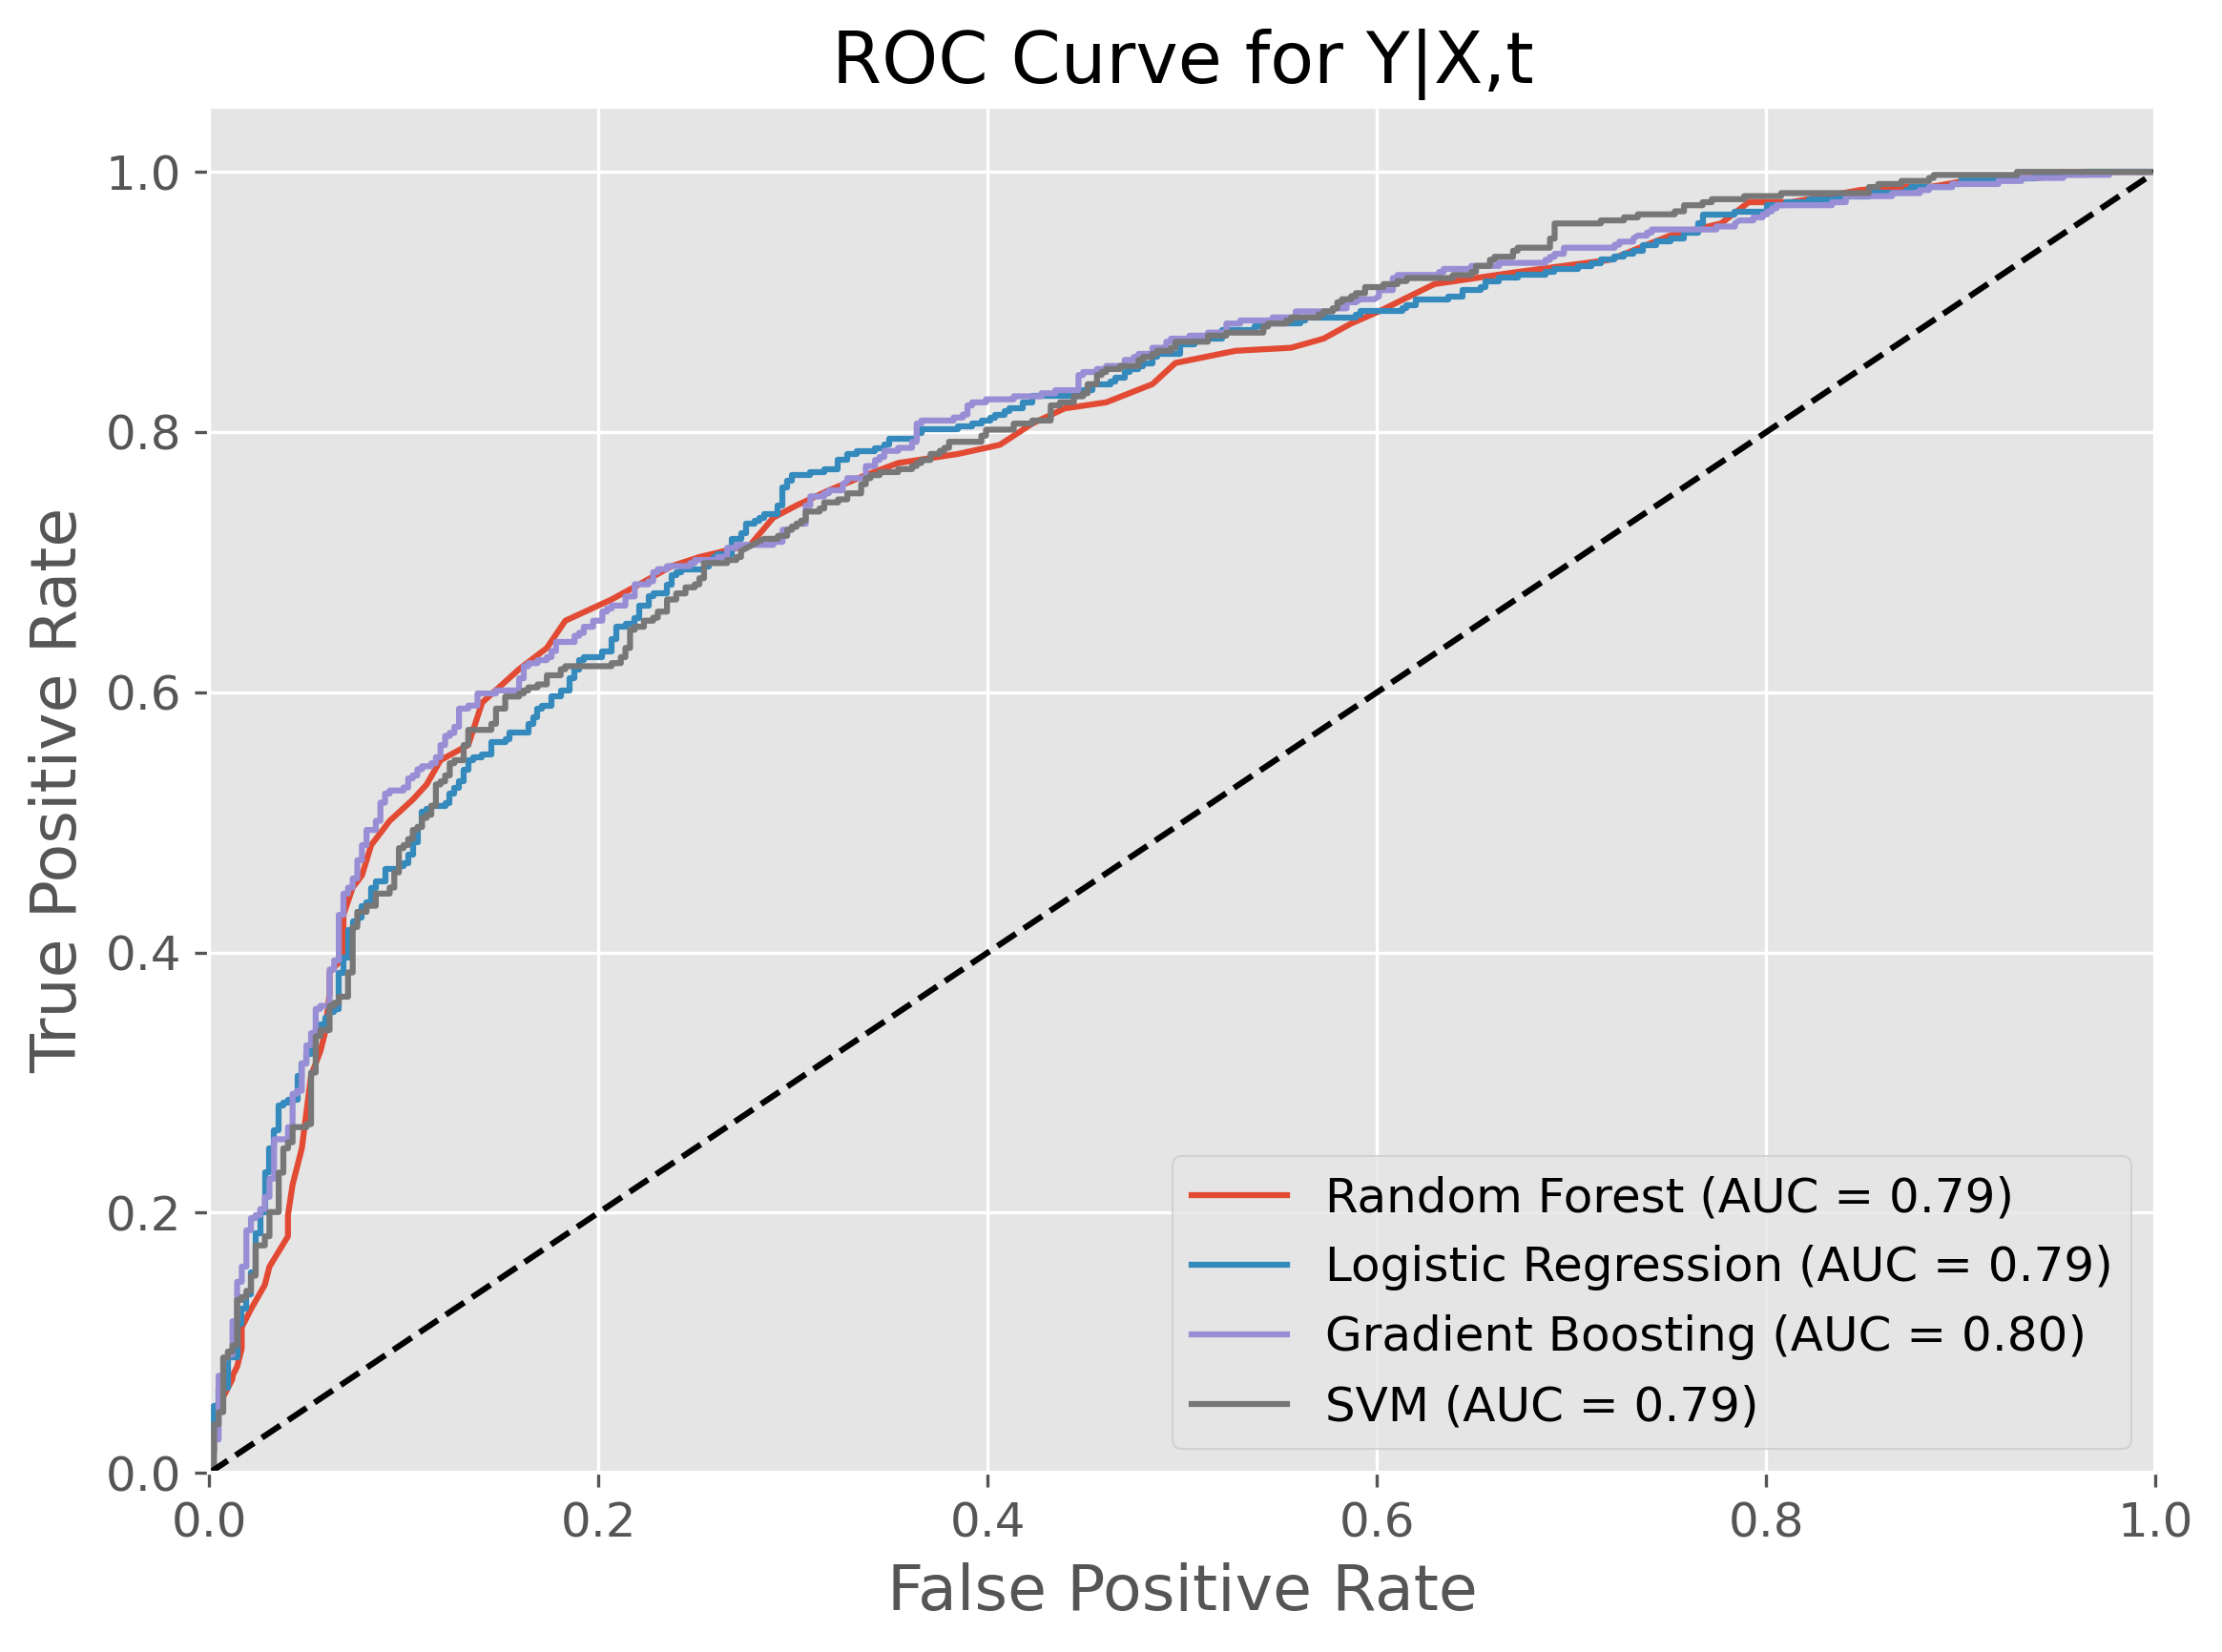
\includegraphics[width=\textwidth]{plots/ROC_curve_Y_given_XT.png}
        \caption{Classifiers of $Y | X, T$}
        \label{fig:ROC_curve_Y_given_XT}
    \end{subfigure}
    \hfill
    \begin{subfigure}[b]{0.45\textwidth}
        \centering
        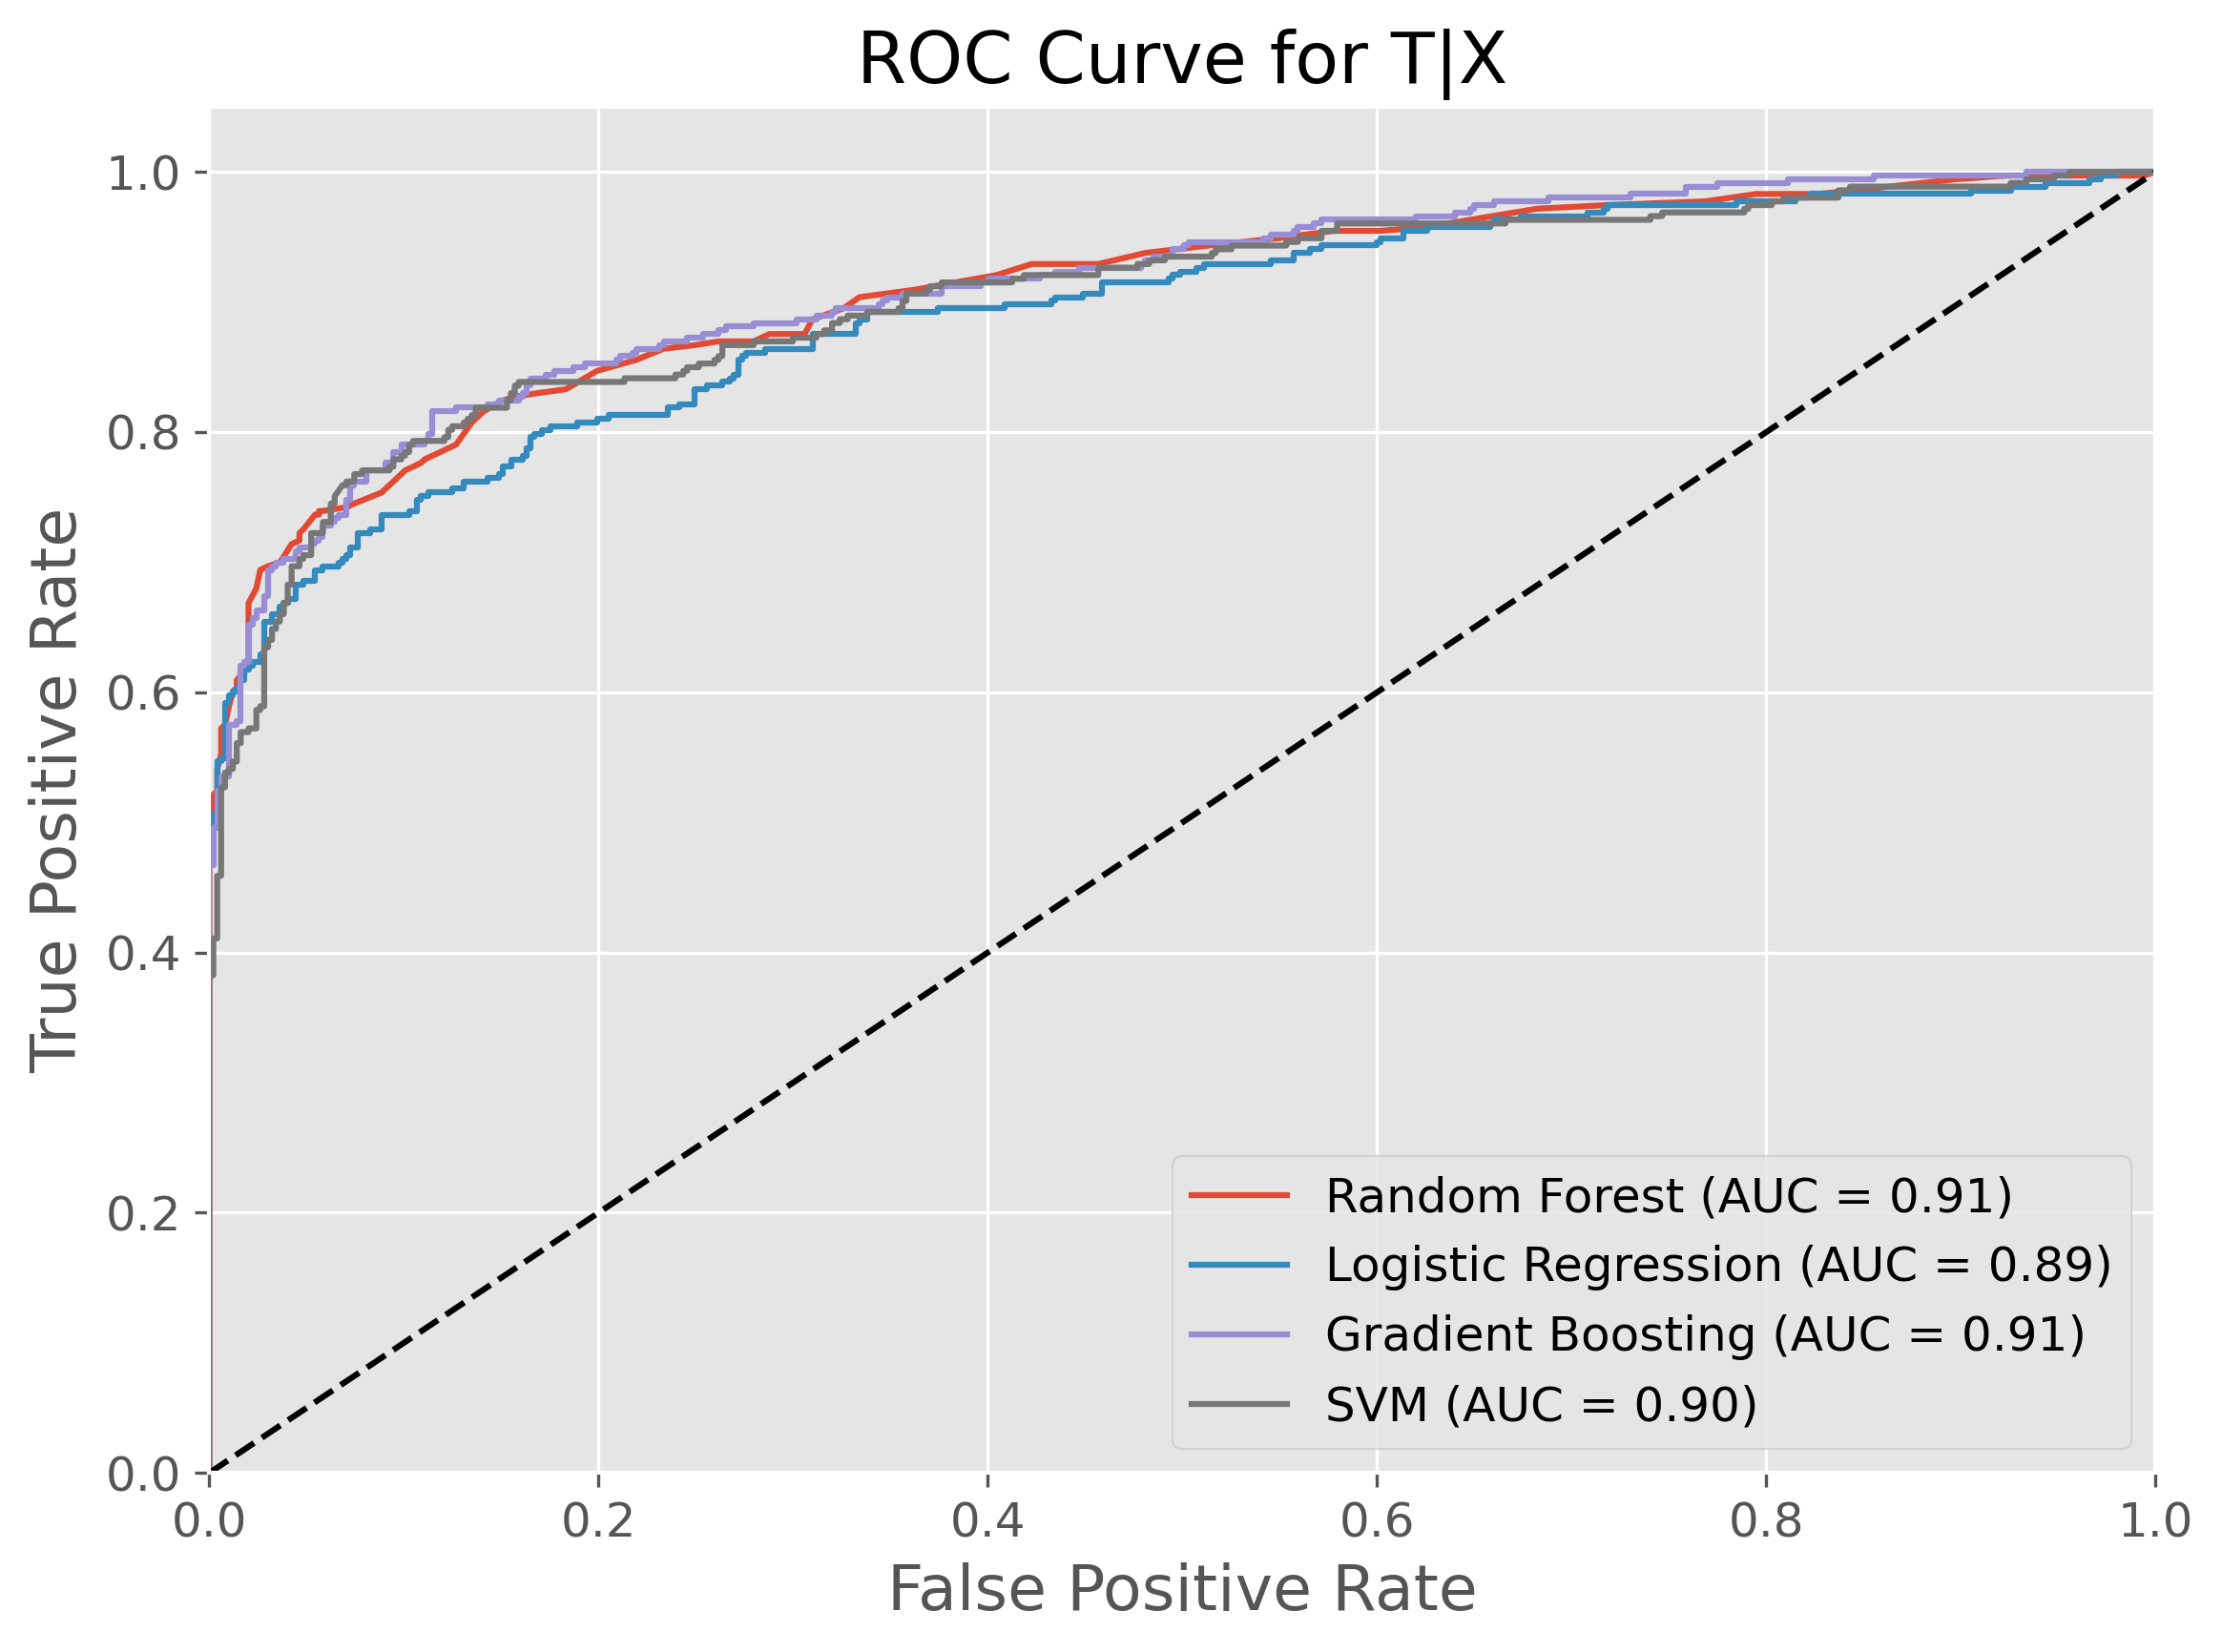
\includegraphics[width=\textwidth]{plots/ROC_curve_T_given_X.png}
        \caption{Classifiers of $T | X$}
        \label{fig:ROC_curve_T_given_X}
    \end{subfigure}
\end{figure}

The fundamental problem of causal inference is that directly observing causal effects is impossible. For any given individual, we can only observe the outcome under one treatment condition - either treated or untreated. We never get to see both potential outcomes for the same unit simultaneously, making it impossible to directly calculate individual treatment effects. In the remainder of this section, we present the estimation methods we used in our analysis, explain how they are trying to handle the mentioned problem, present the assumptions each requires for truthfully estimating the causal effects, and detail the implementation of each method.


% \subsection{Covariate Adjustment}

% Covariate adjustment methods use statistical models to regress the missing potential outcomes based on the observed covariates and the treatment. The regressed values are then used to estimate the average treatment effects.

% There are different covariate adjustment methods, where the separation between them is usually found in if and how to separate the treatment variable from the covariates while regressing the missing potential outcomes and how to use the regressed values for the average effect estimation. We used the methods \emph{S-Learner} and \emph{T-Learner} for our analysis.

% \gur{Theoretical guarantees?}

% \paragraph{S-Learner} Addresses the treatment variable $T$ as one of the covariates. First, one must learn a statistical model for predicting the conditional average treatment effect (CATE) as a function of the covariates $X$ and the treatment $T$ - $\hat{\mu}(X, T) = \hat{\mathbb{E}}[Y^{obs} | X, T]$. Any ML method can be used for this purpose, but importantly, the whole population is used to learn the model. Then, use the learned model to estimate the average treatment effects as follows:

% \begin{itemize}
%     \item \textit{ATE:} Average the predicated causal effect on all of the population:
%     \[
%     \widehat{ATE}^{SL} = \frac{1}{n} \sum_{i=1}^{n} \hat{\mu}(x_i, 1) - \hat{\mu}(x_i, 0)
%     \]
%     \item \textit{ATT:} Average the predicted causal effect on the treatment group:
%     \[
%     \widehat{ATT}^{SL} = \frac{1}{\sum_{i=1}^{n} t_i} \sum \sum_{i=1}^{n} t_i \left[ \hat{\mu}(x_i, 1) - \hat{\mu}(x_i, 0) \right] 
%     \]
%     \item \textit{ATC:} Average the predicted causal effect on the control group:
%     \[
%     \widehat{ATC}^{SL} = \frac{1}{\sum_{i=1}^{n} 1 - t_i} \sum \sum_{i=1}^{n} (1 - t_i) \left[ \hat{\mu}(x_i, 1) - \hat{\mu}(x_i, 0) \right]
%     \]
% \end{itemize}

% \paragraph{T-Learner} Uses observations in the treatment group to estimate the response under control, $\hat\mu_1(x) = \hat{\mathbb{E}}[Y^{obs} | X, 1]$. Similarly, use observations in the control group to estimate the response under treatment, $\hat\mu_0(x) = \hat{\mathbb{E}}[Y^{obs} | X, 0]$. Any machine learning method can be used to get these estimates. Calculating the average effects continues similarly to the S-Learner with $\hat \mu (X_i, T)$ replaced with $\hat \mu_T(x)$.

\subsection{Covariate Adjustment}
Covariate adjustment methods use statistical models to regress the missing potential outcomes based on the observed covariates and the treatment. The regressed values are then used to estimate the average treatment effects.
There are different covariate adjustment methods, where the separation between them is usually found in if and how to separate the treatment variable from the covariates while regressing the missing potential outcomes and how to use the regressed values for the average effect estimation. We used the methods \emph{S-Learner} and \emph{T-Learner} for our analysis.
\paragraph{S-Learner} Addresses the treatment variable $T$ as one of the covariates. First, one must learn a statistical model for predicting the conditional average treatment effect (CATE) as a function of the covariates $X$ and the treatment $T$ - $\hat{\mu}(X, T) = \hat{\mathbb{E}}[Y^{obs} | X, T]$. Any ML method can be used for this purpose, but importantly, the whole population is used to learn the model. Then, use the learned model to estimate the average treatment effects as follows:

\begin{itemize}
    \item \textit{ATE:} Average the predicated causal effect on all of the population:
    \[
    \widehat{ATE}^{SL} = \frac{1}{n} \sum_{i=1}^{n} \hat{\mu}(x_i, 1) - \hat{\mu}(x_i, 0)
    \]
    \item \textit{ATT:} Average the predicted causal effect on the treatment group:
    \[
    \widehat{ATT}^{SL} = \frac{1}{\sum_{i=1}^{n} t_i} \sum_{i=1}^{n} t_i \left[ \hat{\mu}(x_i, 1) - \hat{\mu}(x_i, 0) \right] 
    \]
    \item \textit{ATC:} Average the predicted causal effect on the control group:
    \[
    \widehat{ATC}^{SL} = \frac{1}{\sum_{i=1}^{n} 1 - t_i} \sum_{i=1}^{n} (1 - t_i) \left[ \hat{\mu}(x_i, 1) - \hat{\mu}(x_i, 0) \right]
    \]
\end{itemize}

\citet{hahn1998role} demonstrated that the S-Learner is consistent under the assumptions made in Section~\ref{sec:assumptions} and assuming that the model $\mu(X,T)$ is correctly specified. However, it may be prone to model misspecification, as noted by \citet{rubin1979using}. If the relationship between the covariates and the outcome is incorrectly modeled, it can lead to biased estimates of the treatment effects.

\paragraph{T-Learner} To address the potential issues of model misspecification in the S-Learner, we also employ the T-Learner approach. The T-Learner uses separate models for the treatment and control groups, potentially reducing bias from model misspecification. It uses observations in the treatment group to estimate the response under treatment, $\hat\mu_1(x) = \hat{\mathbb{E}}[Y^{obs} | X, 1]$, and observations in the control group to estimate the response under control, $\hat\mu_0(x) = \hat{\mathbb{E}}[Y^{obs} | X, 0]$. Any machine learning method can be used to get these estimates. Calculating the average effects continues similarly to the S-Learner with $\hat \mu (X_i, T)$ replaced with $\hat \mu_T(x)$.
\citet{greenland1986identifiability} showed that the T-Learner is consistent under the assumptions made in Section~\ref{sec:assumptions} and robust against misspecification of the outcome model. This robustness comes from the separate modeling of the treatment and control groups, which allows for different functional forms in each group.

\paragraph{Implementation Details} We utilized Gradient Boosting classifiers for both the S-Learner and T-Learner approaches. This choice was informed by our analysis of various classifiers' performance in predicting the outcome variable $Y$ given the covariates $X$ and treatment $T$, as illustrated in Figure \ref{fig:ROC_curve_Y_given_XT}. The Gradient Boosting classifier demonstrated the highest Area Under the Curve (AUC) score, indicating its superior predictive performance for our dataset.
For the S-Learner, we trained a single Gradient Boosting model on the entire dataset, including both the covariates and the treatment variable. For the T-Learner, we trained separate Gradient Boosting models for the treated and control groups. We used these models to predict outcomes for all individuals under both treatment conditions in both cases, allowing us to estimate average effects.


\subsection{Propensity-Based Methods}

One of the problems with covariate adjustment methods is the sensitivity to model specification and the sparsity of the covariates when handling high-dimensional data \citep{zhao2020propensity}. The propensity score methods of Rosenbaum and Rubin (RR) aim to address the fundamental problem by adjusting for the propensity score rather than potentially high-dimensional covariates. RR demonstrated that under the assumption of no unmeasured confounding, this is enough for unbiased estimation of causal effects. Such estimation can be accomplished using simple non-parametric methods \citep{abdia2017propensity}.

\paragraph{Inverse Probability Weighting (IPW)} Relies on building a logistic regression model to estimate the probability of the exposure observed (i.e., the propensity score) for a particular individual and using the predicted probability as a weight in subsequent analyses. Our analysis uses the Horvitz–Thompson estimator \citep{horvitz1952generalization}. Intuitively, it estimates the target variable's mean in the treatment and control groups by weighting the observations based on their "membership". One must first train a logistic regression model for predicting the propensity score $\hat e(x) = \hat P(T=1 | X=x)$. Then, use it to weigh each of the samples in the following way to receive each of the average effects:

\begin{itemize}
    \item \textit{ATE:} Compare the weighted means of the treatment and control groups, where units with higher (lower) propensity scores have more influence in the treatment (control) group.
    \[
    \widehat{ATE}^{IPW} = \frac{1}{n}\sum_{i=1}^N \frac{t_i y_i}{\hat e(x)} - \frac{1}{n}\sum_{i=1}^N \frac{(1-t_i)y_i}{1-\hat e(x)}
    \]

    \item \textit{ATT:} Compare the mean of the treatment group with a weighted mean of the control group, where units with higher propensity scores (more likely to be a part of the treatment group) have more influence \citep{lechner2001identification}.
    \[
    \widehat{ATT}^{IPW} = \frac{\sum_{i=1}^N t_i y_i}{\sum_{i=1}^N T_i} - \frac{\sum_{i=1}^N (1-t_i)y_i \cdot \frac{\hat e(x_i)}{1- \hat e(x_i)}}{\sum_{i=1}^N (1-t_i) \cdot \frac{\hat e(x_i)}{1-\hat e(x_i)}}
    \]
    \item \textit{ATC:} Compare the mean of the treatment control with a weighted mean of the treatment group, where units with lower propensity scores (more likely to be a part of the control group) have more influence.
    \[
    \widehat{ATC}^{IPW} = \frac{\sum_{i=1}^N t_iy_i \cdot \frac{1-\hat e(x_i)}{\hat e(x_i)}}{\sum_{i=1}^N t_i \cdot \frac{1-\hat e(x_i)}{\hat e(x_i)}} - \frac{\sum_{i=1}^N (1-t_i)y_i}{\sum_{i=1}^N (1-T_i)}
    \]
\end{itemize}

% \paragraph{Propensity Score Stratification} Divides subjects into strata based on quantiles of their estimated propensity scores \citep{williamson2012propensity}. Subjects with similar propensity scores are placed into the same stratum, ensuring balance within each stratum. 
% It has been shown that stratification with five strata based on the quantiles removes 90\% of the bias in estimating treatment effect \citep{austin2011introduction, rosenbaum1984reducing}.
% Once the strata are created, the treatment effect for each stratum $ \hat{\tau}_k $ is computed as the difference in mean outcomes between treated and control subjects. Formally, for each stratum $ k $, the treatment effect is calculated as $\hat{\tau}_k = \text{Mean}(Y_{T_k}) - \text{Mean}(Y_{C_k})$, where $ \text{Mean}(Y_{T_k}) $ is the average outcome for the treated subjects and $ \text{Mean}(Y_{C_k}) $ is the average outcome for the control subjects in the $ k $-th stratum. \yarden{I would use \(\overline{Y}_{C_k}\) instead of \(\text{Mean}(Y_{C_k})\) and in all other places as well.} The overall causal effects are then calculated by weighting these stratum-specific treatment effects according to the relevant population proportions.

% \begin{itemize}
%     \item \textit{ATE:} Weigh each stratum's treatment effect by the proportion of the total population in that stratum:
%     \[
%     \widehat{ATE}^{STR} = \sum_{k=1}^{K} \frac{N_k}{N} \hat{\tau}_k,
%     \]
%     where $ N_k $ is the number of subjects in the $ k $-th stratum, and $ N $ is the total number of subjects in the entire sample. 

%     \item \textit{ATT:} Weigh each stratum’s treatment effect by the proportion of treated subjects in that stratum:
%     \[
%     \widehat{ATT}^{STR} = \sum_{k=1}^{K} \frac{N_{T_k}}{N_T} \hat{\tau}_k,
%     \]
%     where $ N_{T_k} $ is the number of treated subjects in the $ k $-th stratum, and $ N_T $ is the total number of treated subjects.

%     \item \textit{ATC:} Weigh each stratum's treatment effect by the proportion of control subjects in that stratum:
%     \[
%     \widehat{ATC}^{STR} = \sum_{k=1}^{K} \frac{N_{C_k}}{N_C} \hat{\tau}_k,
%     \]
%     where $ N_{C_k} $ is the number of control subjects in the $ k $-th stratum, and $ N_C $ is the total number of control subjects.
% \end{itemize}

\paragraph{Propensity Score Matching} This method pairs treated units with control units that have similar propensity scores, effectively creating a matched sample where the distribution of observed baseline covariates is similar between treated and untreated subjects \citep{austin2011introduction}. In our implementation, we use a nearest neighbor approach with replacement, allowing for multiple matches per unit. For each unit $i$, we find the $n$ closest matches (where $n = 11$ in our implementation) based on propensity scores. Let $\mathcal{M}i$ denote the set of indices of the $n$ nearest neighbors for unit $i$ in the opposite treatment group. We calculate weights $w_{ij}$ for each match $j \in \mathcal{M}_i$ inversely proportional to the distance in propensity scores 
$w_{ij} = \frac{1/d_{ij}}{\sum_{k \in \mathcal{M}i} 1/d{ik}}$
where $d_{ij}$ is the absolute difference in propensity scores between units $i$ and $j$. The individual treatment effect for unit $i$ is then calculated as
$\tau_i = \begin{cases}
y_i - \sum_{j \in \mathcal{M}i} w_{ij}y_j & \text{if } t_i = 1 \\
\sum_{j \in \mathcal{M}i} w_{ij}y_j - y_i & \text{if } t_i = 0
\end{cases}
$.
The average effects are then calculated as follows:
\begin{itemize}
\item \textit{ATE:} $\widehat{ATE}^{PSM} = \frac{1}{N} \sum_{i=1}^N \tau_i$, where $N$ is the total number of units. This represents the overall average treatment effect for the entire population, calculated by averaging the individual treatment effects over all units, regardless of whether they received the treatment or not.

\item \textit{ATT:} $\widehat{ATT}^{PSM} = \frac{1}{N_1} \sum_{i:t_i=1} \tau_i$, where $N_1$ is the number of treated units. This represents the average treatment effect for the treated group, calculated by averaging the individual treatment effects over all units that received the treatment.

\item \textit{ATC:} $\widehat{ATC}^{PSM} = \frac{1}{N_0} \sum_{i:t_i=0} \tau_i$, where $N_0$ is the number of control units. This represents the average treatment effect for the control group, calculated by averaging the individual treatment effects over all units that did not receive the treatment.

\end{itemize}
This method can be particularly effective in reducing bias due to confounding variables, especially when there is a sufficient overlap in the propensity score distributions between the treated and control groups \citep{rosenbaum1983central}.

\gur{Random forest in propensity, Gradient boosting in $Y$}
\paragraph{Implementation Details} We utilized a Random Forest classifier to estimate the propensity scores. This decision was based on the classifier performance analysis for predicting the treatment assignment (T) given the covariates (X), as shown in Figure \ref{fig:ROC_curve_T_given_X}. The Random Forest classifier exhibited the highest AUC score, indicating its effectiveness in estimating propensity scores for our dataset.
In the IPW method, we used these propensity scores to weight the observations, effectively creating a pseudo-population where the treatment assignment is independent of the measured confounders. We implemented safeguards against extreme propensity scores by clipping the values to a range of [1e-5, 1-1e-5] to prevent issues with very small denominators.
For the Propensity Score Matching method, we employed a nearest neighbor approach with replacement, allowing for multiple matches per unit. We used 11 nearest neighbors for each unit to balance between bias reduction and variance. The matching was performed separately for estimating ATT and ATC, with treated units being matched to control units for ATT, and vice versa for ATC. We calculated weights for each match inversely proportional to the distance in propensity scores, giving more importance to closer matches. This approach allows us to leverage more information from the data compared to one-to-one matching, potentially improving the precision of our estimates while still effectively reducing bias from confounding variables.
\gur{Bootstrap}



\subsection{Doubly-Robust Method}

The doubly robust method fortuitously combines both outcome regression and propensity score weighting, providing a consistent estimator for the average treatment effect even if either the propensity score model or the outcome regression model is misspecified, as long as one of the two is correctly specified \citep{bang2005doubly}. The estimator first requires the estimation of the propensity score, $\hat{e}(x_i)$, and the outcome models, $\hat{\mu}_1(X_i)$ and $\hat{\mu}_0(X_i)$. These are then combined in the following way to estimate the average treatment effects:

\gur{Add explanation of augmentation?}

\begin{itemize}
    \item \textit{ATE:} Compares the weighted and augmented averages of the observed outcomes in the treated and control groups:
    \[
    \widehat{ATE}^{DR} = \frac{1}{N} \sum_i \left( \frac{t_i (y_i - \hat{\mu}_1(x_i))}{\hat{e}(x_i)} + \hat{\mu}_1(x_i) \right) - \frac{1}{N} \sum_i \left( \frac{(1 - t_i)(y_i - \hat{\mu}_0(x_i))}{1 - \hat{e}(x_i)} + \hat{\mu}_0(x_i) \right)
    \]
    
    \item \textit{ATT:} Following \citet{tao2019doubly}, the doubly robust estimator for the ATT compares the observed outcomes in the treated group with a weighted and augmented estimate of the control group's outcomes: 
    \[
    \widehat{ATT}^{DR} = \frac{\sum_i \left[ t_i y_i - \frac{ t_i - \hat{e}(x_i)}{1 - \hat{e}(x_i)} \hat{\mu}_0(x_i) \right]}{\sum_i t_i}
    \]
    
    \item \textit{ATC:} Following \citet{tao2019doubly}, the doubly robust estimator for the ATC compares the observed outcomes in the control group and a weighted and augmented estimate of the treatment group's outcomes:
    \[
    \widehat{ATC}^{DR} = \frac{\sum_i \left[ \{ \frac{ 1 - \hat{e}(x_i)}{\hat{e}(x_i)} t_i y_i - \frac{ t_i - \hat{e}(X_i)}{\hat{e}(X_i)} \hat{\mu}_1(x_i) \}   - (1-t_i)y_i \right]}{\sum_i 1 - t_i}
    \]
\end{itemize}

\paragraph{Implementation Details} We leveraged the strengths of both the outcome regression and propensity score models identified in our previous analyses. We used Gradient Boosting to model the potential outcomes and Random Forest for the propensity score model. This decision is supported by \ref{fig:ROC_curves} and is consistent with the implementation in the previous methods.

\section{Results}

In this section, we present our findings regarding the causal effect of adult enrollment on graduation probability, examining both the relationships between variables through feature importance analysis and the estimated average treatment effects through various methodologies.

\subsection{Feature Importance Analysis}

\begin{figure}
    \centering
    \caption{Important features of classifiers}
    \label{fig:feature_importance}
    \begin{subfigure}[b]{0.45\textwidth}
        \centering
        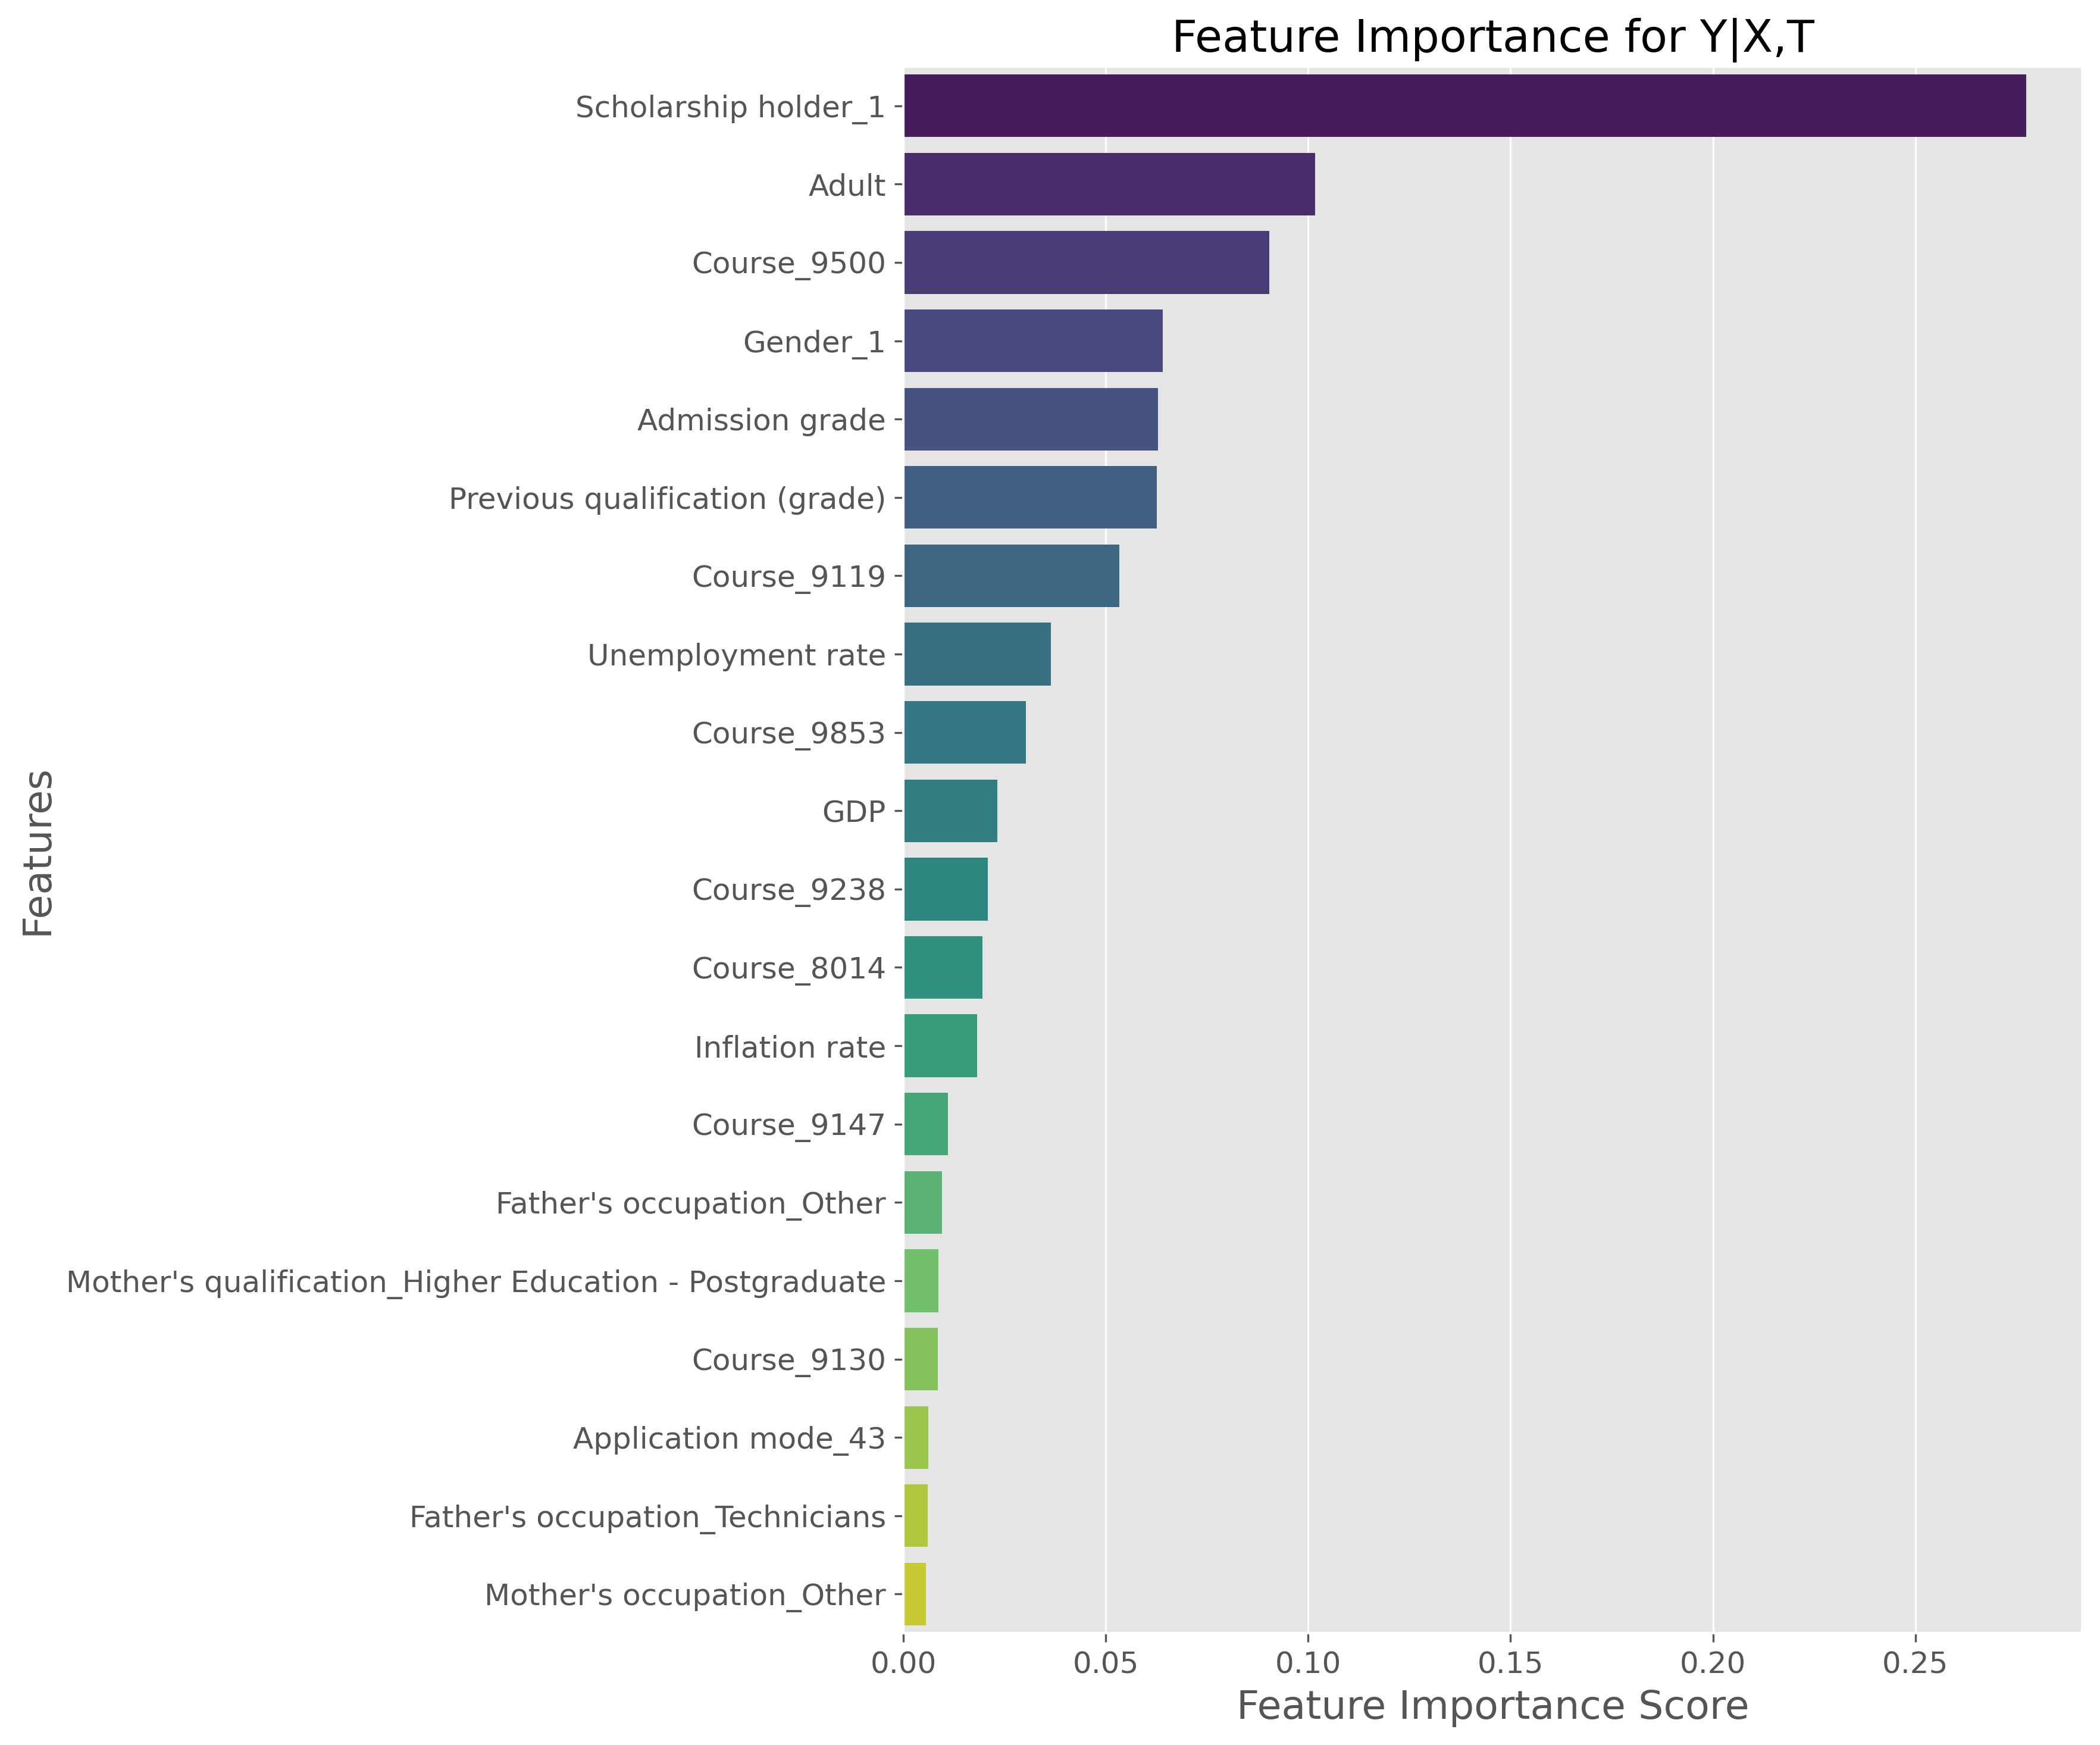
\includegraphics[width=\textwidth]{plots/feature_importance_y_given_xt.png}
        \caption{Feature importance of $Y | X, T$ classifier}
        \label{fig:feature_importance_y_given_xt}
    \end{subfigure}
    \hfill
    \begin{subfigure}[b]{0.45\textwidth}
        \centering
        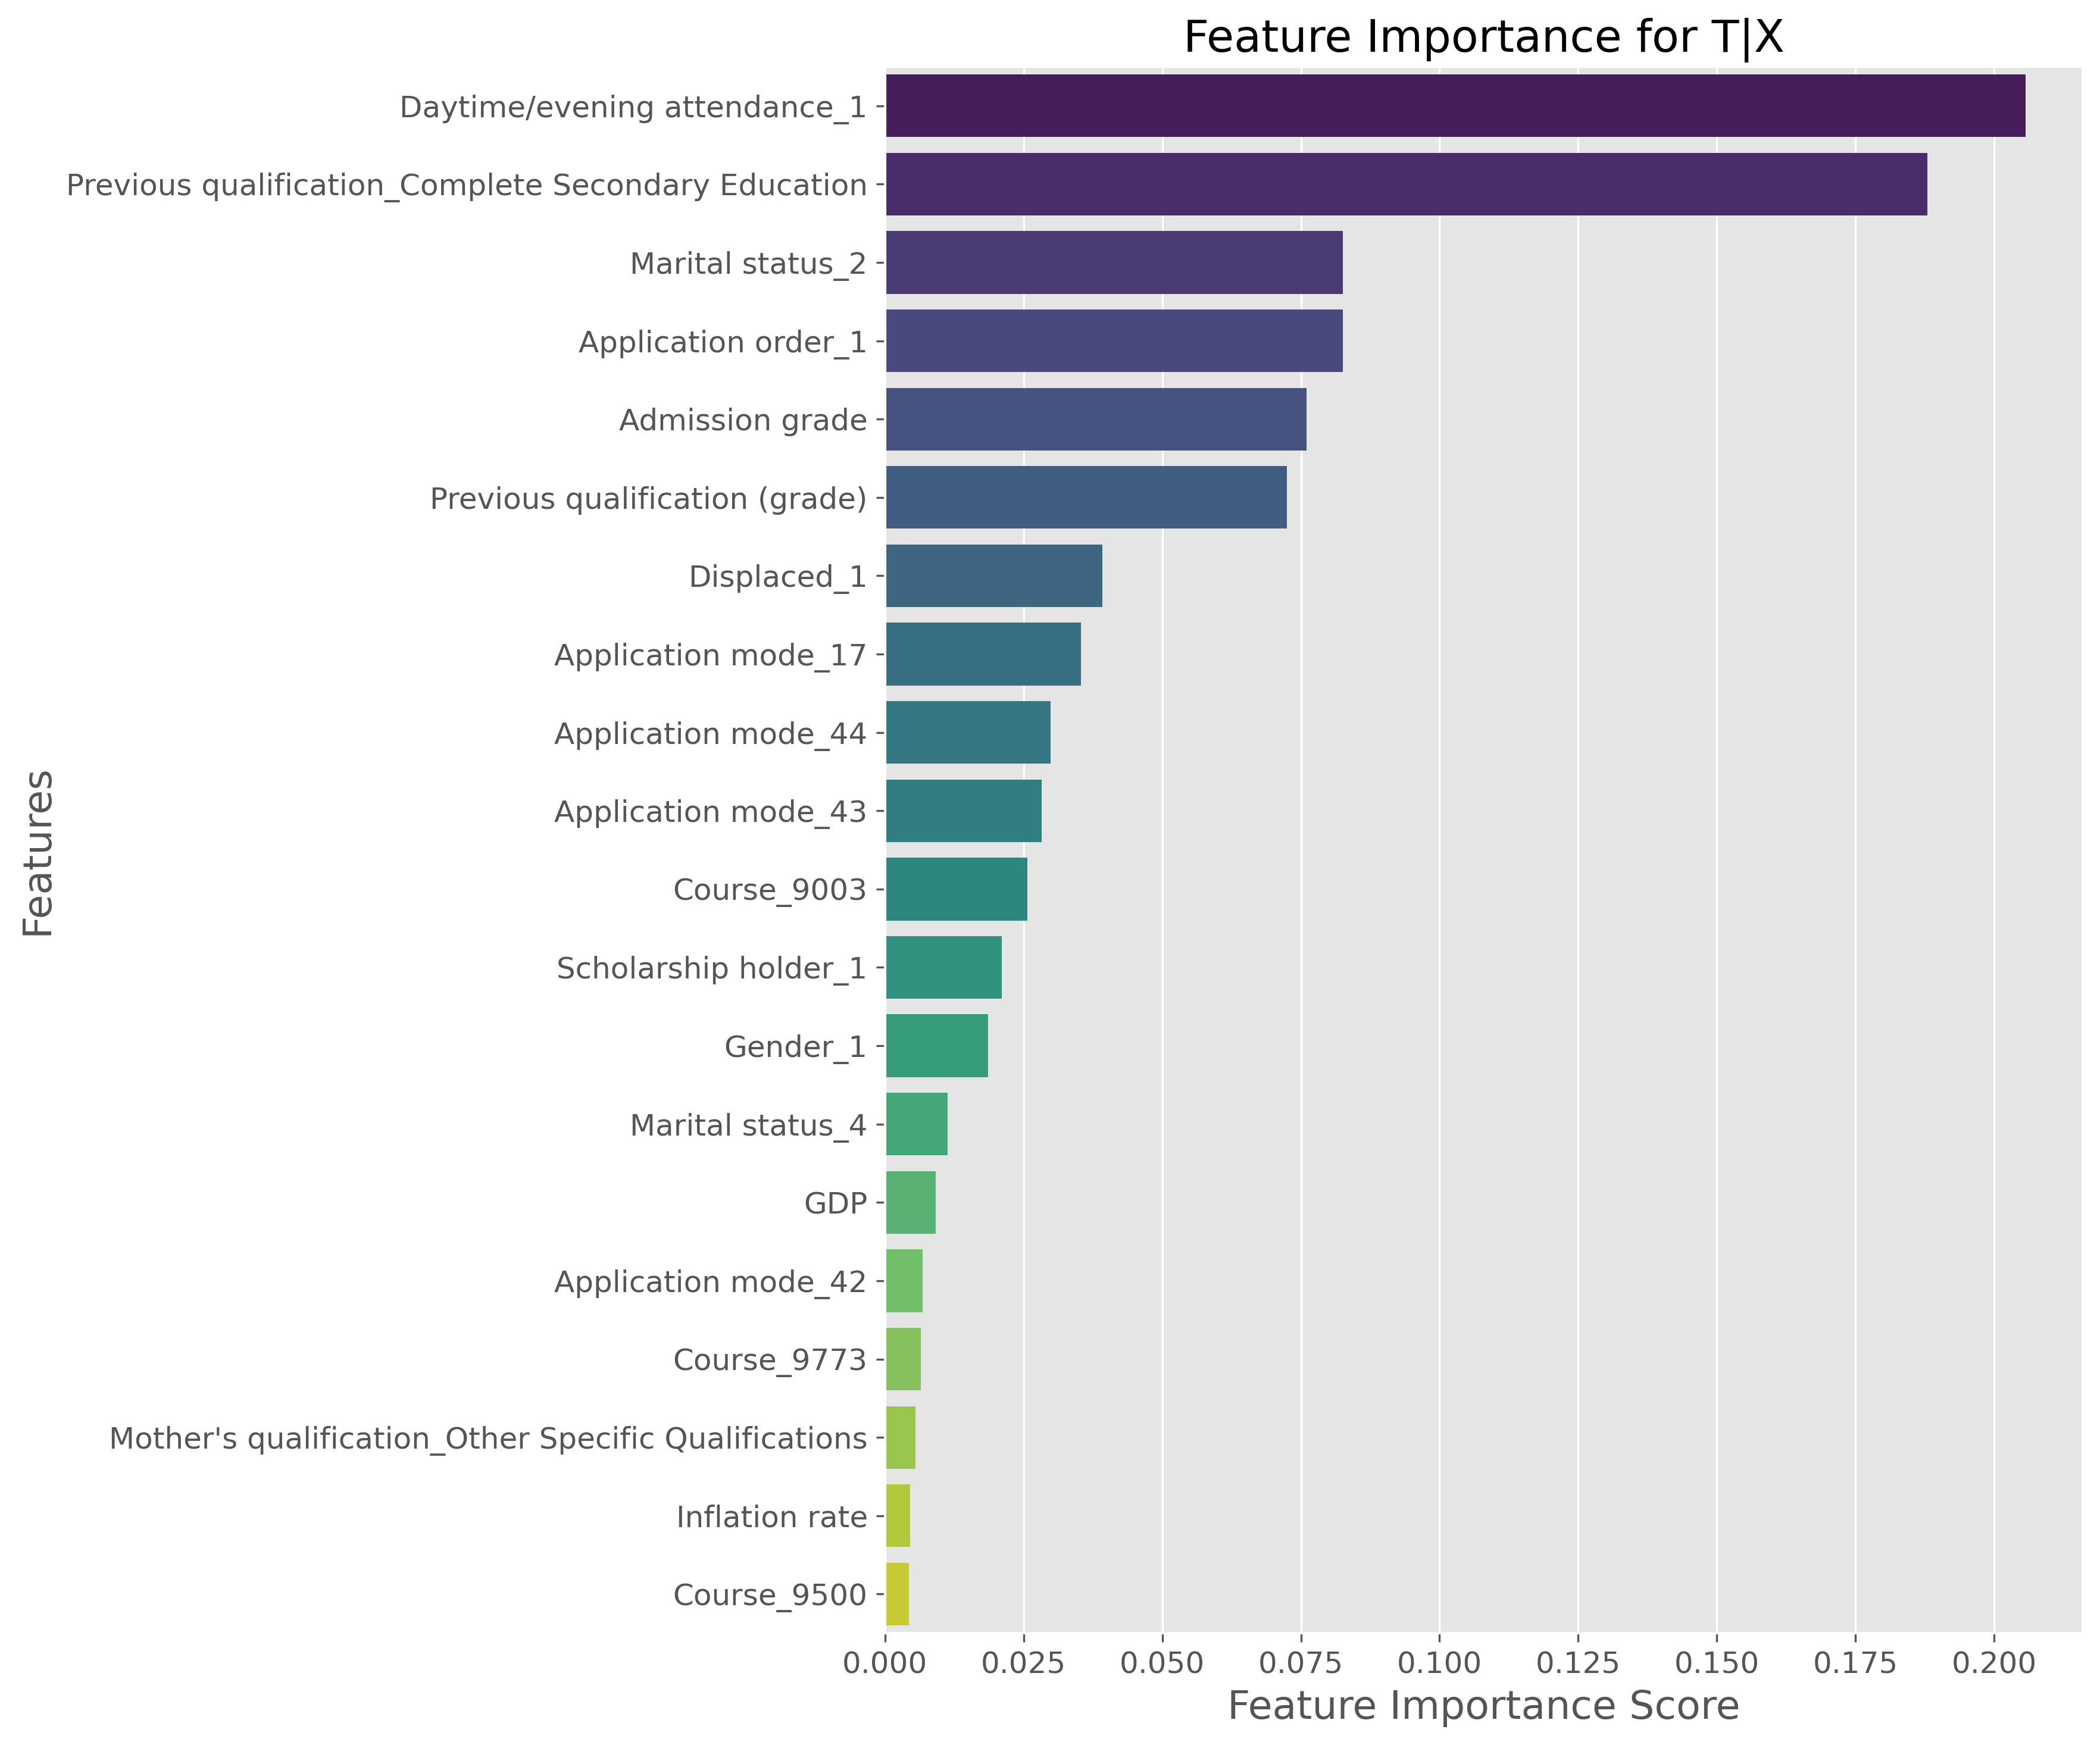
\includegraphics[width=\textwidth]{plots/feature_importance_t_given_x.png}
        \caption{Feature importance of $T | X$ classifier}
        \label{fig:feature_importance_t_given_x}
    \end{subfigure}
\end{figure}

The feature importance analysis was conducted using different approaches for the two classification tasks, as shown in Figure~\ref{fig:feature_importance}. We employed a Random Forest classifier to predict the treatment assignment ($T|X$) and analyzed feature importance using the built-in importance scores based on mean decrease in impurity (Gini importance). We used a Gradient Boosting classifier to predict the outcome given covariates and treatment ($Y|X,T$). We examined its feature importance metrics based on the accumulated reduction in the loss function across all trees.

For the treatment prediction ($T|X$), as illustrated in Figure~\ref{fig:feature_importance_t_given_x}, the most informative features are ``Daytime/evening attendance'' and ``Previous qualification\_Complete Secondary Education'', with importance scores of approximately 0.19 and 0.18 respectively. This suggests these variables strongly correlate with whether a student enrolls as an adult. The application order, marital status, and admission grades also show substantial predictive power for the treatment assignment.

For the outcome prediction ($Y|X,T$), shown in Figure~\ref{fig:feature_importance_y_given_xt}, scholarship holder status emerges as the most informative feature with an importance score of about 0.25. Notably, the treatment variable (``Adult'') appears as the second most informative predictor, with an importance score around 0.12, indicating its strong correlation with graduation outcomes. Course-specific variables (particularly Course\_9500) and gender also demonstrate substantial predictive power. Academic performance indicators such as admission grade and previous qualification grades are also among the top predictive features.

\subsection{Average Effects Analysis}

\begin{figure}
    \centering
    \caption{Box plots of average effects}
    \label{fig:box_plots}
    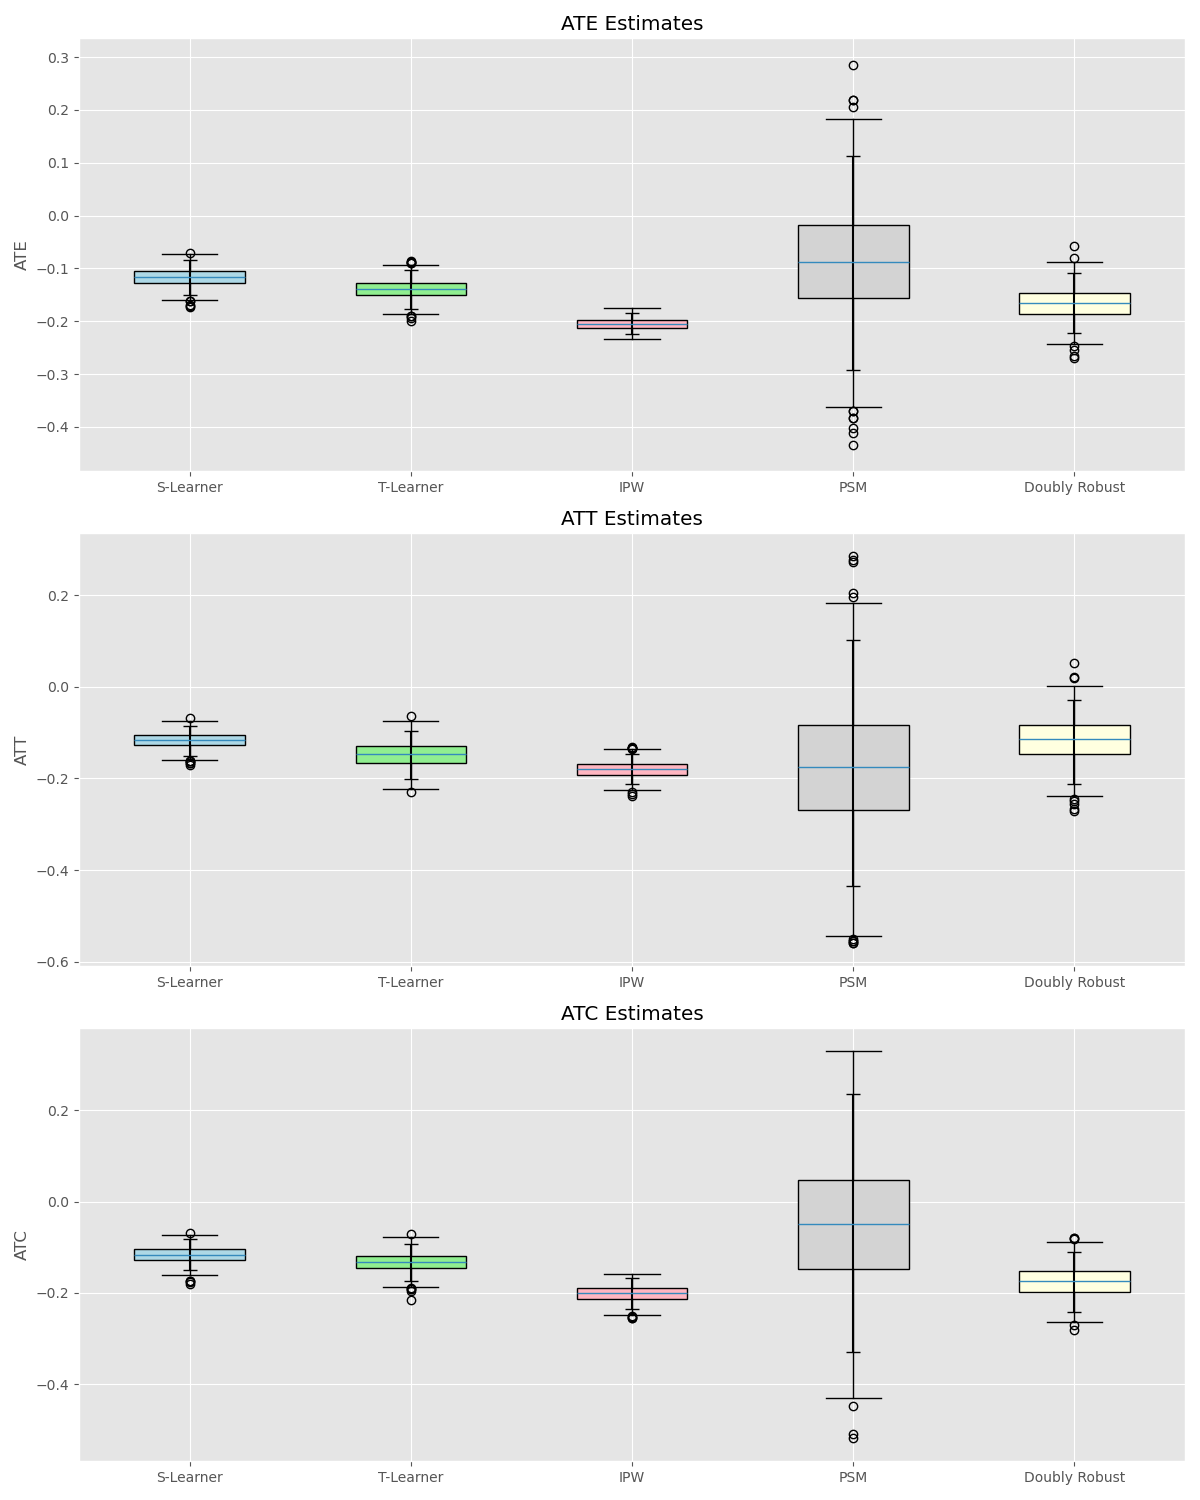
\includegraphics[width = 0.8\textwidth]{plots/box_plots.png}
\end{figure}

The box plots in Figure~\ref{fig:box_plots} reveal consistent patterns across different estimation methods, with some notable variations in both magnitude and uncertainty. For the Average Treatment Effect (ATE), the S-Learner and T-Learner show remarkable agreement, both estimating an effect around $-0.12$ with relatively narrow confidence intervals. The IPW and Doubly Robust estimators also align closely, showing slightly more negative estimates around $-0.15$. While the PSM method shows higher variance, its median estimate remains negative. Importantly, confidence intervals across all methods exclude zero, suggesting a robust negative effect.

The patterns observed in the ATE estimates largely persist in both the ATT and ATC estimates, though with slightly different magnitudes. For both measures, the S-Learner and T-Learner continue to show strong agreement, with estimates around $-0.11$ for ATT and $-0.13$ for ATC. The IPW and Doubly Robust methods estimate slightly more negative effects in both cases. The PSM method consistently shows the highest variance among all methods, with confidence intervals barely including zero in the case of ATC. However, the overall negative trend remains consistent across all methods and measures.

The consistency of negative effects across all three measures (ATE, ATT, and ATC) and most estimation methods provides strong evidence for a negative relationship between adult enrollment and graduation probability. The similarity in magnitude across ATE, ATT, and ATC suggests this relationship is relatively uniform across different subpopulations. While the PSM method shows higher variance, its general alignment with the negative trend supports the robustness of these findings.



\section{Discussion}

\begin{itemize}
    \item Conclusions
    \item Possible weaknesses.
    \item Avenues for future work.
\end{itemize}


\bibliography{references.bib}

\appendix

\newpage
\section{Variables grouped by class}

\begin{table}[h]
\centering
\caption{Attributes used grouped by class of attribute.}
\label{table:variables list}
\begin{tabular}{|l|l|l|}
\hline
\textbf{Class of Attribute}           & \textbf{Attribute}                                                 & \textbf{Type}             \\ \hline
\multirow{6}{*}{Demographic data}     & Marital status                                                     & Numeric/discrete          \\ \cline{2-3} 
                                      & Nationality                                                        & Numeric/discrete          \\ \cline{2-3} 
                                      & Displaced                                                          & Numeric/binary            \\ \cline{2-3} 
                                      & Gender                                                             & Numeric/binary            \\ \cline{2-3} 
                                      & Age at enrollment                                                  & Numeric/discrete          \\ \cline{2-3} 
                                      & International                                                      & Numeric/binary            \\ \hline
\multirow{8}{*}{Socioeconomic data}   & Mother's qualification                                             & Numeric/discrete          \\ \cline{2-3} 
                                      & Father's qualification                                             & Numeric/discrete          \\ \cline{2-3} 
                                      & Mother's occupation                                                & Numeric/discrete          \\ \cline{2-3} 
                                      & Father's occupation                                                & Numeric/discrete          \\ \cline{2-3} 
                                      & Educational special needs                                          & Numeric/binary            \\ \cline{2-3} 
                                      & Debtor                                                             & Numeric/binary            \\ \cline{2-3} 
                                      & Tuition fees up to date                                            & Numeric/binary            \\ \cline{2-3} 
                                      & Scholarship holder                                                 & Numeric/binary            \\ \hline
\multirow{3}{*}{Macroeconomic data}   & Unemployment rate                                                  & Numeric/continuous        \\ \cline{2-3} 
                                      & Inflation rate                                                     & Numeric/continuous        \\ \cline{2-3} 
                                      & GDP                                                                & Numeric/continuous        \\ \hline
\multirow{5}{*}{Academic data at enrollment} & Application mode                                                   & Numeric/discrete          \\ \cline{2-3} 
                                      & Application order                                                  & Numeric/ordinal           \\ \cline{2-3} 
                                      & Course                                                             & Numeric/discrete          \\ \cline{2-3} 
                                      & Daytime/evening attendance                                         & Numeric/binary            \\ \cline{2-3} 
                                      & Previous qualification                                             & Numeric/discrete          \\ \hline
\multirow{6}{*}{Academic data at the end of 1st semester} & Curricular units 1st sem (credited)                                & Numeric/discrete          \\ \cline{2-3} 
                                      & Curricular units 1st sem (enrolled)                                & Numeric/discrete          \\ \cline{2-3} 
                                      & Curricular units 1st sem (evaluations)                             & Numeric/discrete          \\ \cline{2-3} 
                                      & Curricular units 1st sem (approved)                                & Numeric/discrete          \\ \cline{2-3} 
                                      & Curricular units 1st sem (grade)                                   & Numeric/continuous        \\ \cline{2-3} 
                                      & Curricular units 1st sem (without evaluations)                     & Numeric/discrete          \\ \hline
\multirow{6}{*}{Academic data at the end of 2nd semester} & Curricular units 2nd sem (credited)                                & Numeric/discrete          \\ \cline{2-3} 
                                      & Curricular units 2nd sem (enrolled)                                & Numeric/discrete          \\ \cline{2-3} 
                                      & Curricular units 2nd sem (evaluations)                             & Numeric/discrete          \\ \cline{2-3} 
                                      & Curricular units 2nd sem (approved)                                & Numeric/discrete          \\ \cline{2-3} 
                                      & Curricular units 2nd sem (grade)                                   & Numeric/continuous        \\ \cline{2-3} 
                                      & Curricular units 2nd sem (without evaluations)                     & Numeric/discrete          \\ \hline
Target                               & Target                                                             & Categorical               \\ \hline
\end{tabular}
\end{table}





\end{document}